
La dependencia de los combustibles fósiles trae consigo problemas como la inseguridad energética y el incremento de gases de efecto invernadero. Las sociedades que concentran la producción de los combustibles fósiles podrían controlar geopolítica y económicamente a otras \cite{mayer2022fossil}, esta inseguridad energética se evidenció en la crísis del petróleo de 1973 \cite{vernon1976oil} y en la disputa entre Rusia y la Unión Europea por el suministro de gas en el 2022 \cite{rodriguez2022improving}. En contraste, el problema del incremento de la temperatura global es un problema más discreto en los medios de información pero no menos alarmante. En el 2018, la \textit{Intergovernmental Panel on Climate Change} (IPCC) emitió un informe sobre los impactos que causaría dicho incremento en 1.5°C con respecto a los niveles preindustriales para el 2040, que en resumidas cuentas prevé un detrimento crítico y sin retorno de la civilización y la biósfera \cite{guilyardi2018ipcc}. A fin de hacer frente a estos problemas, la transición hacia una matriz energética mundial donde predominen fuentes energéticas menos contaminantes y descentralizadas es la solución. 

Las fuentes renovables reunen dichas características, por lo que muchos gobiernos y organizaciones han tomado acciones para aprovecharlas. En ese marco, la \textit{International Renewable Energy Agency} (IRENA) realizó un análisis multisectorial en el 2020 donde propuso una hoja de ruta para que las energías renovables generen el 86\% de la electricidad global \cite{asmelash2020role}. En ese documento también se menciona que esta cifra no se alcanzaría sin la investigación ni el desarrollo de tecnologías que aprovechen dichas fuentes para hacerlas sostenibles y comercialmente viables.


Hace un año, la energía hidroeléctrica generó más de 4 mil tera-vatios por hora (TWh) en el mundo, lo que representó más del 50\% de la generación de todas las renovables \cite{irena2022international}. No obstante, construir centrales hidroeléctricas favorecería solo a los países con ríos en zonas montañosas. Sin contar esta fuente, las energías eólica y solar son las que encabezan la producción energética. Con el propósito de contextualizar 

en el 2021, y que su vez
es mayor que el total de potencia consumida por las otras energías renovables, cerca de 3.5 mil TWh, no es rentable la construcción de centrales 
hidroeléctricas en diversos territorios a diferencia de las termoeléctricas. En contraste a esta situación, las otras fuentes son menos costosas de implementar y sus unidades
de generación energética son modulables pero el reto actual es incrementar su potencia de generación y su adptación en el mercado. Entre dichas fuentes, resaltan la energía eólica y solar 
estas son las que más porcentaje de potencia de consumo han tenido  en el 2021 a nivel mundial, pero la energía solar es la que más crecimiento mostró sobre todo en sudamérica y el Perú
 (ver Figura \ref{img:PorcentajeRenovable}). Este hecho puede deberse a causas políticas, económicas y tecnológicas; pero hace evidente que serán una fuente renovable no hídricas preponderante en los próximos años. 

\begin{figure}[h]
    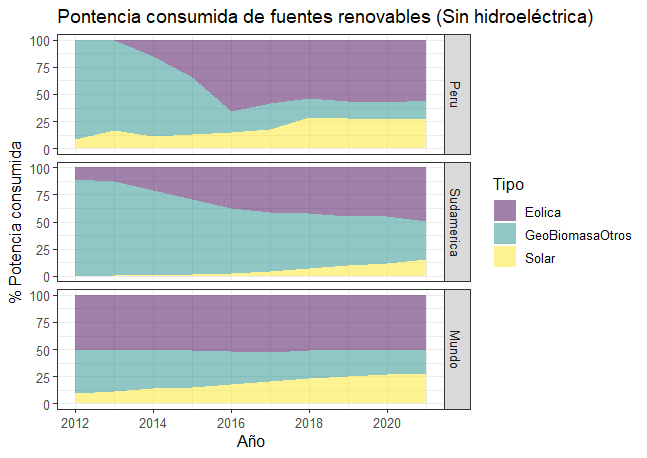
\includegraphics[scale=0.8]{img/PorcentajeRenovable.png}
    \caption{Comparación del porcentaje de la cantidad de potencia consumida por tipo de energía renovable sin considerar la hidroeléctrica.
    Fuente: Our World in Data \cite{owidenergy}}
    \label{img:PorcentajeRenovable}
\end{figure}

La energía solar es accesible para las personas en todos los terrenos habitables y gracias a los 140 mil TWh/h que el sol genera se considera una fuente casi ilimitada \cite{hammarstrom2012}.
Sin embargo, el aprovechamiento de esta energía requiere de dispositivos que deben ser capáces de capturar, transformar 
y almacenar la mayor cantidad de energía lumínica en trabajo útil en rangos de tiempo variantes a causa del tiempo atmosférico y
los estadíos solares.


Existen dos tipos de tecnlogías que aprovechan la energía solar: La termosolar y la fotovoltaica. En la tecnología termosolar se condensa el haz solar en un contenedor de un fluído de tal manera que este se caliente
y mueva un alternador eléctrico, mientras que la energía fotovoltaica convierte la radiación solar en energía electroquímica directamente 
por medio de fenómenos fotovoltaicos que se ocurren dentro de los materiales .
Las centrales termosolares tienen el potencial de generar miles de kilos-vatios por hora (KWh) no obstante 
existen desventajas que limitan la difusión de su uso tales como su alto costo en la instalación, mantenimiento y distribución por cableado 
eléctrico, así como la gran cantidad de energía desperdiciada en los procesos de transferencia de calor. Estos problemas están casi ausentes
en los sistemas fotovoltaicos ya que se usan paneles y modulos que facilitan su uso, sin embargo aún es un reto equiparar la eficiencia de estos dispositivos con los termosolares. Si bien existen tecnologías que unen la termosolar y fotovoltaica, el presente trabajo se enfoca en mejorar los dispositivos fotovoltaicos.

Las celdas solares, centros funcionales de los sistemas fotovoltaicos, llevan en el mercado más de 60 años, desde su descubrimiento en los  Laboratorios Bell en 1954 \cite{green2009path} y su primer uso comercial en el satélite Vanguard \cite{singh2013solar}. En términos de impacto ambiental, los sistemas fotovoltaicos generan entre 14 a 73 gr-$CO_2$/kWh, lo cual es casi 90\% menos del impacto que generan los sistemas basados en gas \cite{tawalbeh2021environmental}. Gracias 

Blakers cita a la 
\textit{National Renewable Energy Labotatories} (NREL) con el propósito de describir la clasificación que esta institución hace a varios tipos de celdas  según los mejores rendimientos que mostraron en sus fases experimentales \cite{blakers2013}, por otro lado Rathore y su equipo se basaron en la antigûedad comercial y madurez técnica de estas \cite{rathore2021}. Por fines prácticos se hace uso de esta última para describir las tres generaciones que engloban varios tipos de celdas así como sus características principales. 

En la primera generación están las celdas construídas a base de obleas de silicio monocristalinas y policristalinas. Las monocristalinas han alcanzado rendimientos mayores al 20\% \cite{gul2016}, no obstante su fabricación es costosa  \cite{srinivas2015review} debido al "recristalizado" de silicio por el método de Czochralski \cite{yu2019growth} para formar lingotes de monocristal que luego se cortan. Frente a esto, el uso de diferentes policristales en las celdas abarató el costo gracias a que se fabrican con procesos de enfriamiento simples, además sus eficiencias de conversión energética oscilan de entre 12-14\%, por lo que estas características le permiten ser el tipo de celda con más prevalencia en el mercado \cite{sharma2015solar}. 

En la segunda generación se encuentran las celdas en base películas delgadas de silicio amorfo (a-Si) \cite{kaur2016review}, cadmio-teluro (CdTe) \cite{bertolli2008} y cobre-indio-galio-selenio (CIGS) \cite{bagher2015types}, la característica principal de estas celdas es que son económicas en comparación con las de otras generaciones \cite{rathore2021}, sin embargo sus limitaciones son la inestabilidad de la eficiencia \cite{gul2016review} así como los impactos negativos en el ambiente y a la salud que causan sus materiales, como el cadmio por ejemplo \cite{bagher2015types}. 

Finalmente, la tercera generación agrupa a las celdas más recientes tales como aquellas basadas en concentradores, nano cristales, polímeros y sensibilizadas por tintes. Las celdas por concentradores son dispositivos rígidos que aprovechan la radiación y el calor que se generan en al incidir luz en lentes convexos \cite{bertolli2008}, si bien tiene viabilidad comercial se demandan mejoras en los materiales fotovoltaicos. Las celdas basadas en nano cristales o \textit{quantum dots} (QD) pueden capturar mejor la luz mientras suprimen fenómenos de recombinación además de tener un rendimiento estable por encima del 20\% \cite{kim2022conformal}, no obstante no son comercialmente viables porque son costosos de fabricar \cite{jean2018synthesis}. Por el contrario, las celdas de polímero se caracterizan por su flexibilidad pero sus rendimientos estan en promedio por debajo del 10\% y a su vez son inestables porque son sensibles a cambios de temperatura y presión \cite{gusain2019polymer}. Por último, las celdas sensibilizadas por tintes son dispositivos que tienen semiconductores fotosensibilizados y ensamblados a un sistema electrolítico que permite un flujo continuo de electrones \cite{suhaimi2015materials}, se caracterizan por su construcción versátil y de bajo costo gracias a la diversidad materiales de sus componentes, sin embargo sus rendimientos aún no se equiparan a las comerciales de silicio \cite{sharma2018dye}. 


Las celdas sensibilizadas por tintes (CSPT) pueden ser 

$\dots$ debido a todas estas razones, la investigación de nuevos materiales y procesos de fabricación para celdas solares sensibilizadas por tintes más costo eficientes cobran relevancia. 


Las estructura de las celdas solares 


Es claro que deben de validarse experimentalmente los resultados obtenidos por los métodos compuacionales, pero estos pueden discriminar cientos de candidat


pero dado un grado de precisión razonable  en la predicción de la propiedad del material, estos modelos computcionales aceleran el proceso de elegir mejores estructuras o moléculas candidatas con la correcta combinación de propiedades necesarias para cumplir satisfactoriamente con el propósito para las que fueron hechas \textit{Leon R. Devereux}. 



